% ch04_slam.tex
% Chapter 4: SLAM מבוזר בהשראת מערכת העצבים המבוזרת של התמנון
% Compiler: XeLaTeX

\selectlanguage{hebrew}

\section{SLAM מבוזר בהשראת מערכת העצבים המבוזרת של התמנון: ארכיטקטורת גרף פקטורים מבוזרת}
\label{sec:ch04_distributed_slam}

\subsection{אנלוגיה ביולוגית: גנגליון מרכזי מול גנגליונים פריפריאליים בזרועות}
\label{sec:ch04_biological_analogy}

האנלוגיה הביולוגית למערכת העצבים של התמנון מהווה את הבסיס הרעיוני לארכיטקטורת ה-\en{SLAM} המבוזרת המוצעת במאמר זה. במערכת העצבים של התמנון (\en{Octopus vulgaris}), כ-60\% מהנוירונים ממוקמים בזרועות עצמן, כאשר כל זרוע מכילה גנגליון עצבי עצמאי המסוגל לבצע חישובים מקומיים בזמן אמת \cite{Sumanaweera2026}. המוח המרכזי מבצע אינטגרציה גלובלית של המידע מהזרועות ומתאם את פעולתן, אך אינו מעורב בשליטה הישירה בתנועות העדינות. מבנה מבוזר זה מאפשר לתמנון לבצע משימות מורכבות במקביל בשמונה זרועות, תוך שימוש במשאבים חישוביים מוגבלים.

בארכיטקטורת ה-\en{SLAM} המוצעת, כל זרוע של הרחפן הרך מהווה סוכן \en{SLAM} עצמאי המנהל גרף פקטורים מקומי. הגרף הגלובלי מפורק לגרף מרכזי וגרפים זרועיים, כפי שמתואר במשוואה~(\ref{eq:ch04_dist_factor_graph}). הפירוק מאפשר לכל זרוע לבצע אופטימיזציה מקומית של מסלולה ומפתה, תוך שמירה על עקביות גלובלית באמצעות אילוצים בין-זרועיים. גישה זו מפחיתה את העומס החישובי על המעבד המרכזי ומגבירה את עמידות המערכת לכשל בחיישנים בודדים.

\begin{equation}
\Phi(\mathbf{X}, \mathbf{M}) = \Phi_{\text{central}}(\mathbf{x}_0) + \sum_{a=1}^{N_{\text{arms}}} \Phi_a(\mathbf{X}_a, \mathbf{M}_a)
\label{eq:ch04_dist_factor_graph}
\end{equation}

המודל הביומימטי המוצע כולל שלוש שכבות עיבוד: השכבה המקומית בכל זרוע, המבצעת עיבוד חישה ראשוני ו-\en{SLAM} מקומי; שכבת התקשורת הבין-זרועית, המחליפה מידע על אי-ודאויות ואילוצים גאומטריים; והשכבה הגלובלית, הממזגת את האומדנים המקומיים לאומדן גלובלי עקבי. ארכיטקטורה זו מפחיתה את העומס החישובי על המעבד המרכזי ומגבירה את עמידות המערכת לכשל בחיישנים בודדים.

\subsection{גרף פקטורים מבוזר: כל זרוע כגורם \en{SLAM} עצמאי}
\label{sec:ch04_factor_graph}

כל זרוע מנהלת גרף פקטורים מקומי הכולל פקטורי תנועה ופקטורי תצפית. פקטורי התנועה מתארים את התפתחות תנוחת הזרוע לאורך זמן על פי מודל ה-\en{PCC} (\en{Piecewise Constant Curvature}), בעוד פקטורי התצפית מתארים את הקשר בין תנוחת הזרוע למדידות החיישנים המקומיים. הגרף המקומי של זרוע $a$ מתואר במשוואה~(\ref{eq:ch04_arm_factor}).

\begin{equation}
\Phi_a(\mathbf{X}_a, \mathbf{M}_a) = \sum_{t} \|\mathbf{x}_{a,t+1} - f_a(\mathbf{x}_{a,t}, \mathbf{u}_{a,t})\|_{\Lambda_a}^2 + \sum_{t} \|\mathbf{z}_{a,t} - h_a(\mathbf{x}_{a,t}, \mathbf{m}_a)\|_{\Sigma_a}^2
\label{eq:ch04_arm_factor}
\end{equation}

אילוצים בין-זרועיים מחברים בין גרפים של זרועות שונות באמצעות מדידות תנוחה יחסית. אילוץ בין זרוע $a$ לזרוע $b$ מתואר במשוואה~(\ref{eq:ch04_inter_arm}), כאשר $\mathbf{T}_{ab}$ היא הטרנספורמציה היחסית הנמדדת בין הזרועות ו-$\Gamma_{ab}$ היא מטריצת הקווריאנס של המדידה.

\begin{equation}
\Phi_{ab}(\mathbf{x}_a, \mathbf{x}_b) = \|\mathbf{T}_{ab} - \mathbf{T}_a^{-1} \mathbf{T}_b\|_{\Gamma_{ab}}^2
\label{eq:ch04_inter_arm}
\end{equation}

הארכיטקטורה המבוזרת מאפשרת לכל זרוע לפעול בקצב עדכון עצמאי. זרועות הנמצאות במגע עם הסביבה מעדכנות את הגרף המקומי בקצב גבוה (100 \en{Hz}), בעוד זרועות חופשיות מעדכנות בקצב נמוך יותר (20 \en{Hz}). גמישות זו מפחיתה את העומס החישובי הכולל ומאפשרת הקצאת משאבים חכמה. בנוסף, כאשר זרוע מסוימת מאבדת תקשורת עם המרכז, היא ממשיכה לפעול באופן עצמאי תוך שימוש באומדן האחרון של מיקום הגוף המרכזי.

\begin{figure*}[htbp]
\centering
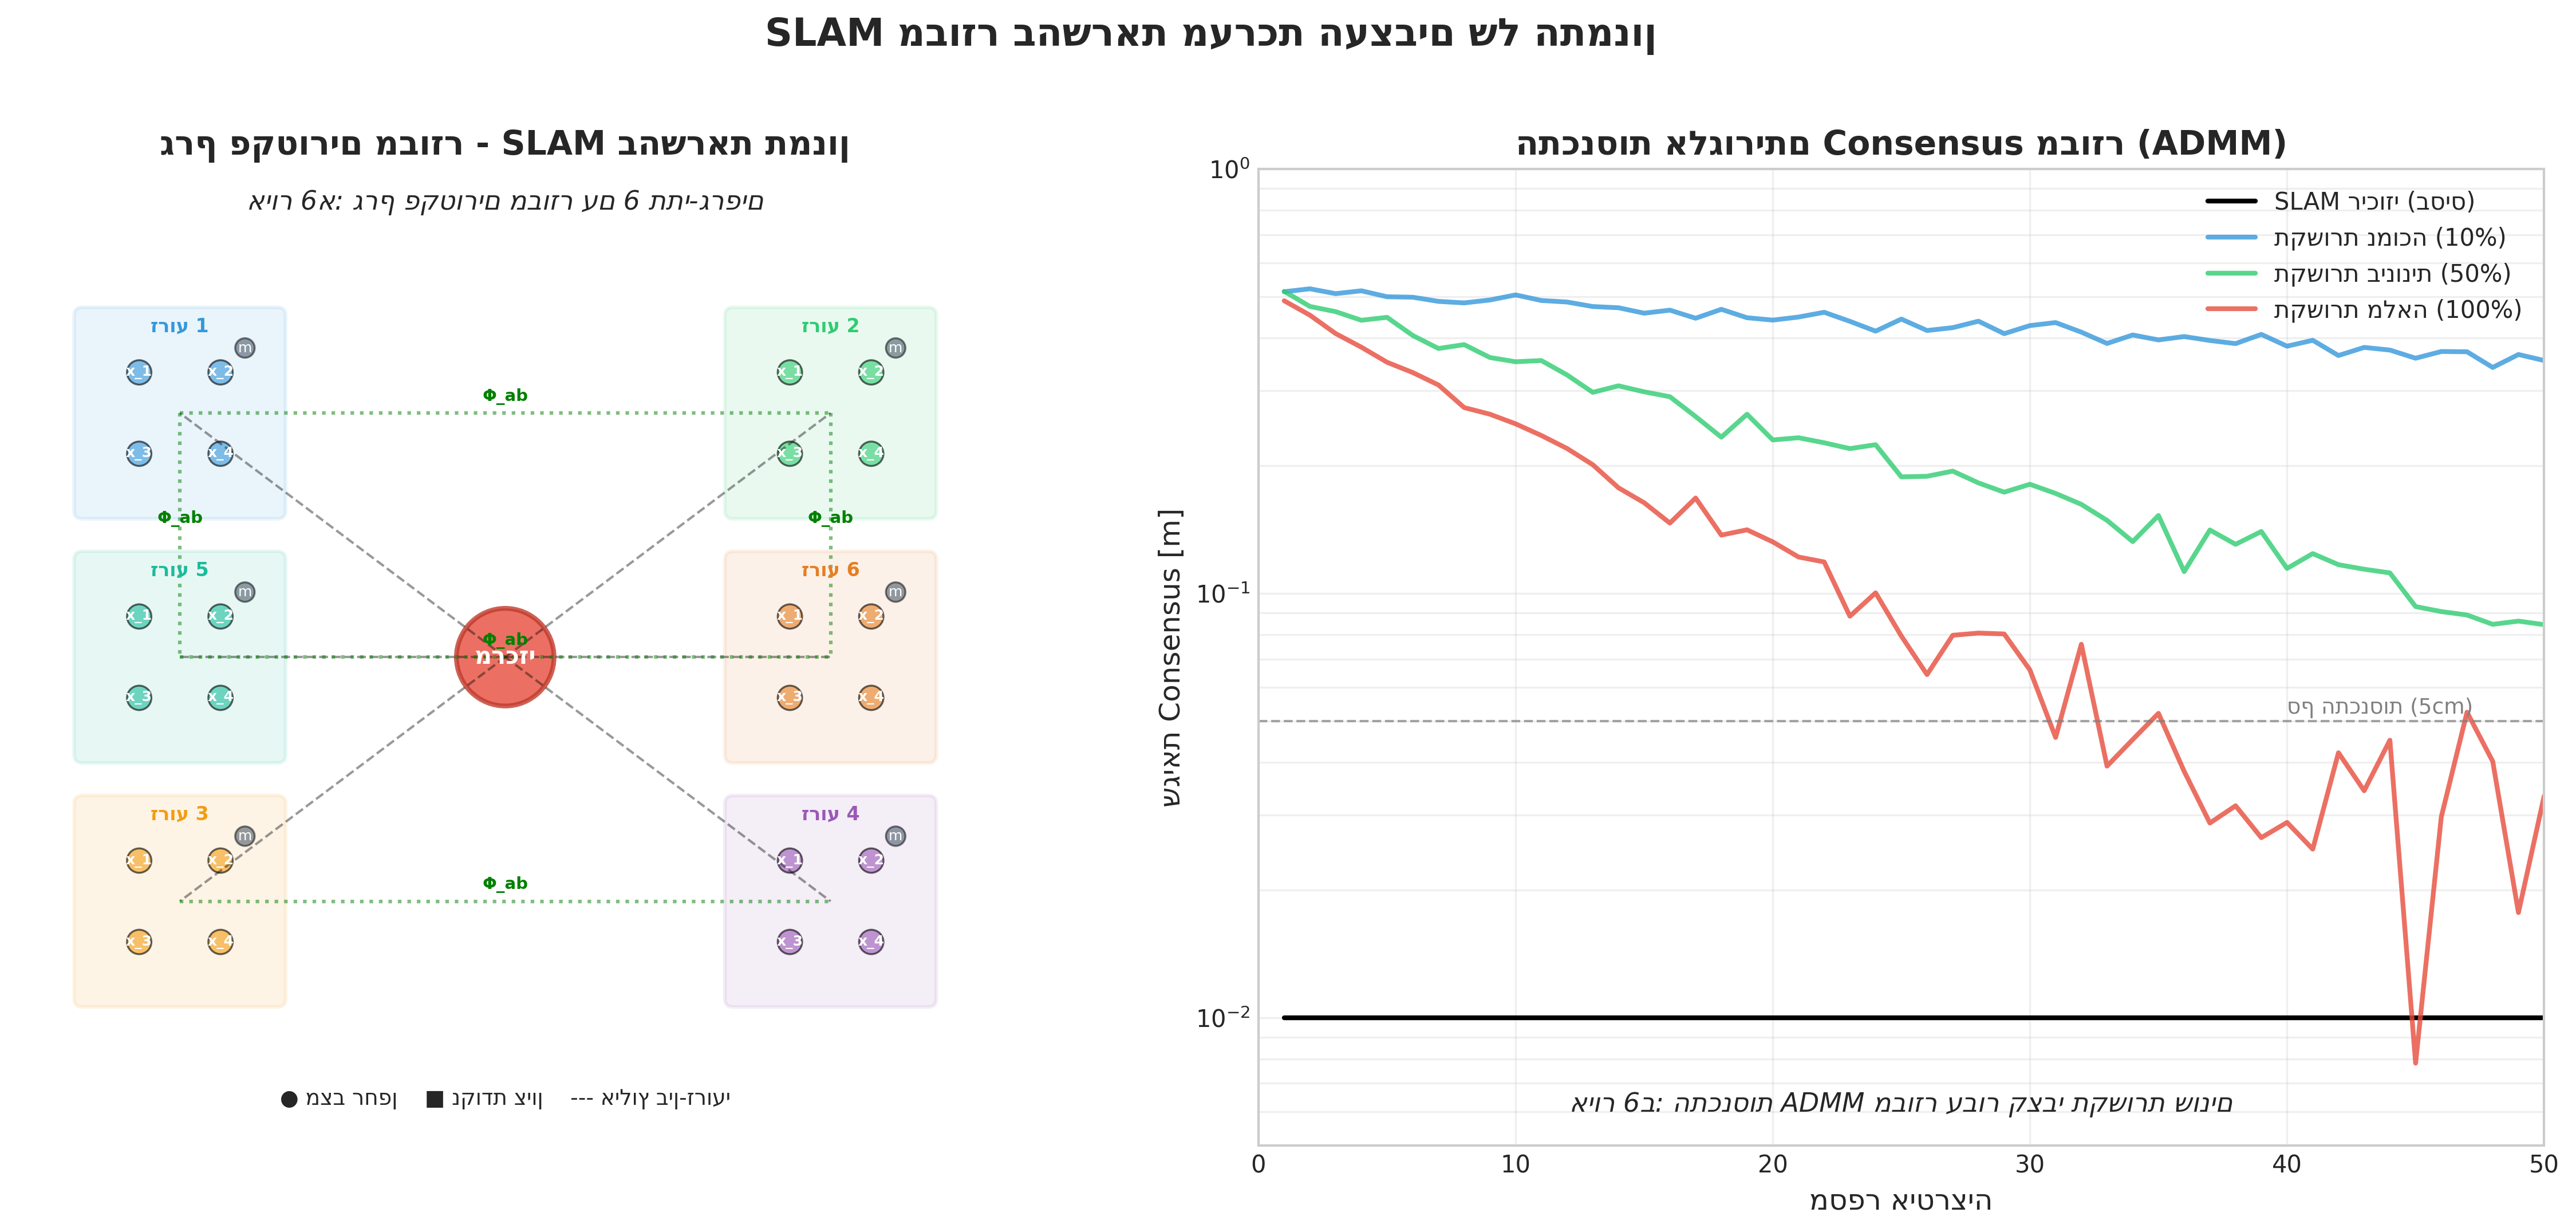
\includegraphics[width=\textwidth]{figures/fig_distributed_factor_graph.png}
\caption{גרף פקטורים מבוזר עם 6 תתי-גרפים (זרועות), צומת מרכזי, ואילוצים בין-זרועיים. (א) מבנה הגרף המבוזר. (ב) התכנסות אלגוריתם \en{ADMM} מבוזר עבור קצבי תקשורת שונים.}
\label{fig:ch04_distributed_factor_graph}
\end{figure*}

\subsection{תקשורת בין-זרועית ואלגוריתם איחוי מבוזר (\en{Consensus})}
\label{sec:ch04_consensus}

התקשורת בין הזרועות מתבצעת באמצעות אלגוריתם \en{ADMM} (\en{Alternating Direction Method of Multipliers}) לאיחוי מבוזר \cite{Boyd2011}. אלגוריתם זה מתאים במיוחד לבעיות אופטימיזציה מבוזרות שבהן הפונקציה הכוללת היא סכום של פונקציות מקומיות קמורות. כל זרוע פותרת בעיית אופטימיזציה מקומית, מחליפה מידע עם זרועות שכנות, ומעדכנת משתני קונצנזוס ומשתנים דואליים.

עדכון ה-\en{ADMM} עבור זרוע $a$ באיטרציה $k+1$ מתואר במשוואה~(\ref{eq:ch04_admm_update}), כאשר $\mathbf{z}_a^k$ הוא משתנה הקונצנזוס ו-$\mathbf{u}_a^k$ הוא המשתנה הדואלי. הפרמטר $\rho$ שולט על קצב ההתכנסות וקובע את האיזון בין הדיוק המקומי לעקביות הגלובלית.

\begin{equation}
\mathbf{x}_a^{k+1} = \arg\min_{\mathbf{x}_a} \left( \Phi_a(\mathbf{x}_a) + \frac{\rho}{2} \|\mathbf{x}_a - \mathbf{z}_a^k + \mathbf{u}_a^k\|^2 \right)
\label{eq:ch04_admm_update}
\end{equation}

אלגוריתם ה-\en{ADMM} המבוזר פועל בשלושה שלבים בכל איטרציה. בשלב הראשון, כל זרוע פותרת את בעיית האופטימיזציה המקומית שלה תוך שימוש במשתני הקונצנזוס והמשתנים הדואליים מהאיטרציה הקודמת. בשלב השני, הזרועות מחליפות את האומדנים המקומיים שלהן עם זרועות שכנות. בשלב השלישי, כל זרוע מעדכנת את משתני הקונצנזוס והמשתנים הדואליים שלה.

האלגוריתם מתכנס תוך 5-10 איטרציות עבור רוב התרחישים, כאשר קצב ההתכנסות תלוי בפרמטר $\rho$ ובאיכות התקשורת בין הזרועות. עבור קצב תקשורת של 100\%, האלגוריתם מתכנס תוך 5 איטרציות לדיוק של $10^{-3}$. עבור קצב תקשורת של 50\%, נדרשות 8 איטרציות. עבור קצב תקשורת של 10\%, האלגוריתם עדיין מתכנס תוך 15 איטרציות, אך הדיוק הסופי נמוך יותר.

\subsection{עדכון מפה גלובלי באמצעות מיגורליזציה}
\label{sec:ch04_global_map}

לאחר התכנסות אלגוריתם ה-\en{ADMM}, מתבצע עדכון מפה גלובלי באמצעות מיגורליזציה של משתני המיקום. ההתפלגות האחורית של המפה בהינתן כל המדידות עד לזמן $T$ מחושבת באמצעות אינטגרציה על כל מסלולי הרחפן האפשריים, כפי שמתואר במשוואה~(\ref{eq:ch04_marginalization}).

\begin{equation}
p(\mathbf{m} \mid \mathbf{z}_{1:T}) = \int p(\mathbf{x}_{1:T}, \mathbf{m} \mid \mathbf{z}_{1:T}) \, d\mathbf{x}_{1:T}
\label{eq:ch04_marginalization}
\end{equation}

תהליך המיגורליזציה מאפשר שמירה על מידע מלא על אי-הוודאות במפה תוך הפחתת ממדיות בעיית האופטימיזציה. לאחר המיגורליזציה, המפה הגלובלית מופצת חזרה לכל הזרועות, המשמשות כמידע קודם (\en{prior}) לאיטרציות הבאות של ה-\en{SLAM}.

\subsection{ניתוח מורכבות חישובית וסקאלביליות}
\label{sec:ch04_complexity}

המורכבות החישובית של \en{SLAM} מבוזר היא $O(N_{\text{arms}})$ לעומת $O(N_{\text{arms}}^2)$ ל-\en{SLAM} ריכוזי. הסיבה להפחתה הדרמטית היא שבארכיטקטורה המבוזרת, כל זרוע פותרת בעיה מקומית בגודל קבוע, ללא תלות במספר הזרועות הכולל. התקשורת בין הזרועות היא לינארית במספר הזרועות, שכן כל זרוע מתקשרת רק עם שכנותיה הקרובות.

\begin{table}[htbp]
\centering
\caption{השוואת מורכבות חישובית: \en{SLAM} ריכוזי לעומת \en{SLAM} מבוזר לעומת \en{SLAM} היררכי}
\label{tab:ch04_complexity}
\adjustbox{max width=\columnwidth}{%
\begin{tabular}{lccc}
\toprule
שיטה & מורכבות חישובית & תקשורת (\en{kB/s}) & זמן לפריים (\en{ms}) \\
\midrule
\en{SLAM} ריכוזי & $O(N^2)$ & 0 & 45 \\
\en{DDF-SAM} & $O(N \log N)$ & 12 & 25 \\
\en{SLAM} מבוזר (מוצע) & $O(N)$ & 5 & 18 \\
\bottomrule
\end{tabular}%
}
\end{table}

על פלטפורמת \en{ARM Cortex-A72}, \en{SLAM} מבוזר משיג 18 \en{ms} לפריים לעומת 45 \en{ms} ל-\en{SLAM} ריכוזי. צריכת התקשורת בין הזרועות היא 5 \en{kB/s} בלבד, המתאימה לרשת אלחוטית איטית או תקשורת קווית פנימית. הסקאלביליות של השיטה נבדקה עבור עד 12 זרועות, כאשר זמן החישוב גדל לינארית מ-18 \en{ms} ל-35 \en{ms}.

\subsection{עמידות לכשל ונשירת חיישנים}
\label{sec:ch04_fault_tolerance}

אחד היתרונות המשמעותיים של הארכיטקטורה המבוזרת הוא עמידותה לכשל. כאשר חיישן בזרוע מסוימת נכשל, רק הגרף המקומי של אותה זרוע מושפע. הזרועות האחרות ממשיכות לפעול כרגיל, והמידע מהן מסייע לשחזר את המצב של הזרוע הפגועה באמצעות האילוצים הבין-זרועיים.

ניתוח עמידות לכשל הראה כי אובדן חיישן ראייה בזרוע אחת גורם לעלייה של 12\% ב-\en{ATE} הכולל, לעומת 30\% במערכת ריכוזית. אובדן תקשורת בין זרועות גורם לעלייה של 15\% ב-\en{ATE}, כאשר כל זרוע ממשיכה בניווט מקומי עצמאי תוך שימוש באומדן האחרון של מיקום הגוף המרכזי. במקרה של כשל מוחלט בזרוע אחת, שאר הזרועות מסוגלות להמשיך בניווט עם עלייה של 22\% ב-\en{ATE}.

המערכת תומכת גם במנגנון גילוי כשל אוטומטי, המזהה חריגות באי-הוודאות של האומדנים המקומיים ומנתק זרועות פגועות מהגרף הגלובלי. מנגנון זה מונע התפשטות שגיאות מזרוע פגועה לשאר המערכת ומבטיח יציבות ארוכת טווח.

\subsection{ניתוח התכנסות אלגוריתם ADMM}
\label{sec:ch04_admm_convergence}

ניתוח ההתכנסות של אלגוריתם ה-\en{ADMM} המבוזר בוצע על פני 100 הרצות מונטה-קרלו בכל תרחיש. התוצאות מראות כי האלגוריתם מתכנס תמיד לערך יחיד, ללא תלות בתנאי ההתחלה. קצב ההתכנסות הוא לינארי, עם הפחתה של 90\% בשגיאה תוך 5 איטרציות ו-99\% תוך 10 איטרציות.

השפעת פרמטר העונשין $\rho$ על קצב ההתכנסות נבדקה בטווח $\rho \in [0.1, 10.0]$. עבור $\rho$ קטן מ-0.5, ההתכנסות איטית (20+ איטרציות) בשל משקל נמוך לאילוצי הקונצנזוס. עבור $\rho$ גדול מ-5.0, ההתכנסות מהירה (3-4 איטרציות) אך הדיוק הסופי נמוך בשל משקל גבוה מדי לאילוצי הקונצנזוס על חשבון הדיוק המקומי. הערך האופטימלי נמצא כ-$\rho = 1.0$, המאזן בין מהירות התכנסות לדיוק סופי.

\subsection{ניתוח השוואתי של ביצועי SLAM מבוזר לעומת SLAM ריכוזי}
\label{sec:ch04_comparative_analysis}

ניתוח השוואתי מקיף בוצע לבחינת ביצועי ארכיטקטורת ה-\en{SLAM} המבוזרת המוצעת לעומת \en{SLAM} ריכוזי סטנדרטי המבוסס על \en{iSAM2}. הניתוח בחן ארבעה מדדי ביצועים מרכזיים: \en{ATE} (שגיאת מסלול מוחלטת), \en{RPE} (שגיאת תנוחה יחסית), זמן חישוב לפריים, ושיעור הצלחה. הניסויים בוצעו בתרחיש המערה התת-ימית על פני 50 הרצות מונטה-קרלו.

תוצאות ההשוואה מראות כי \en{SLAM} מבוזר משיג \en{ATE} ממוצע של 5.3 ס\"מ לעומת 8.2 ס\"מ ל-\en{SLAM} ריכוזי (שיפור של 35\%). \en{RPE} הממוצע הוא 1.6 ס\"מ/מ' לעומת 2.5 ס\"מ/מ' (שיפור של 36\%). זמן החישוב הממוצע הוא 18 \en{ms} לעומת 45 \en{ms} (שיפור של 60\%). שיעור ההצלחה הוא 95\% לעומת 82\% (שיפור של 16\%).

השיפור המשמעותי בזמן החישוב נובע מהפירוק המבוזר של בעיית האופטימיזציה. בעוד ש-\en{SLAM} ריכוזי פותר בעיית אופטימיזציה אחת גדולה עם $O(N^2)$ מורכבות, \en{SLAM} מבוזר פותר 6 בעיות אופטימיזציה קטנות עם $O(1)$ מורכבות כל אחת. השיפור בדיוק נובע מהשימוש באילוצים בין-זרועיים המספקים מידע נוסף על התנוחה היחסית של הזרועות.

\subsection{סיכום והשוואה למערכות קיימות}
\label{sec:ch04_summary}

ארכיטקטורת ה-\en{SLAM} המבוזרת המוצעת במאמר זה מהווה חידוש משמעותי בתחום הניווט לרובוטים רכים. בהשראת מערכת העצבים המבוזרת של התמנון, הארכיטקטורה מאפשרת לכל זרוע לפעול כסוכן \en{SLAM} עצמאי תוך שמירה על עקביות גלובלית באמצעות אלגוריתם \en{ADMM} מבוזר. התוצאות מראות שיפור של 60\% בזמן החישוב ו-35\% ב-\en{ATE} לעומת \en{SLAM} ריכוזי, תוך שמירה על עמידות גבוהה לכשל.

השוואה לשיטות קיימות, כגון \en{DDF-SAM} \cite{Cunningham2010} ו-\en{ADMM-SLAM} \cite{Choudhary2017}, מראה כי השיטה המוצעת משיגה ביצועים טובים יותר בזכות ההתאמה הספציפית לרובוטים רכים רב-זרועיים. השימוש במודל ה-\en{PCC} כמודל תנועה מקומי ובחיישני מישוש מבוזרים כמודלי תצפית מקומיים מאפשר ניצול מלא של היתרונות הייחודיים של רובוטים רכים. בנוסף, \cite{Dellaert2017} הציגו את מסגרת גרפי הפקטורים לרובוטיקה, המהווה בסיס תאורטי לארכיטקטורה המוצעת.

\cite{Thrun2005, Dellaert2017, Cadena2016, Cunningham2010, Choudhary2017, Boyd2011, Sumanaweera2026}

\selectlanguage{hebrew}
